\subsection{Dopaminerges System}
\label{dopaminerges_system}
%%%%%%%%%%%%%%%%%%%%%%%%%%%%%%%%
\index{System! dopaminerg}
Das Catecholamin Dopamin\index{Dopamin} (Abb.~\ref{fig:dopamin}) wird ausgehend von der aromatischen Aminosäure Tyrosin synthetisiert. Der Großteil des Dopamins wird in rostralen Nuclei, der Substantia nigra \index{Substantia nigra} und der VTA des Mesencephalons, gebildet. Es können zwischen vier größeren dopaminergen Nerventrakten unterschieden werden. Drei von ihnen entspringen dem Mesencephalon (Abb.~\ref{dopaminerges_system}) \textsuperscript{\cite[Kap.~13]{kandel2013principles}}. 


\begin{figure}[H]
    \centering
    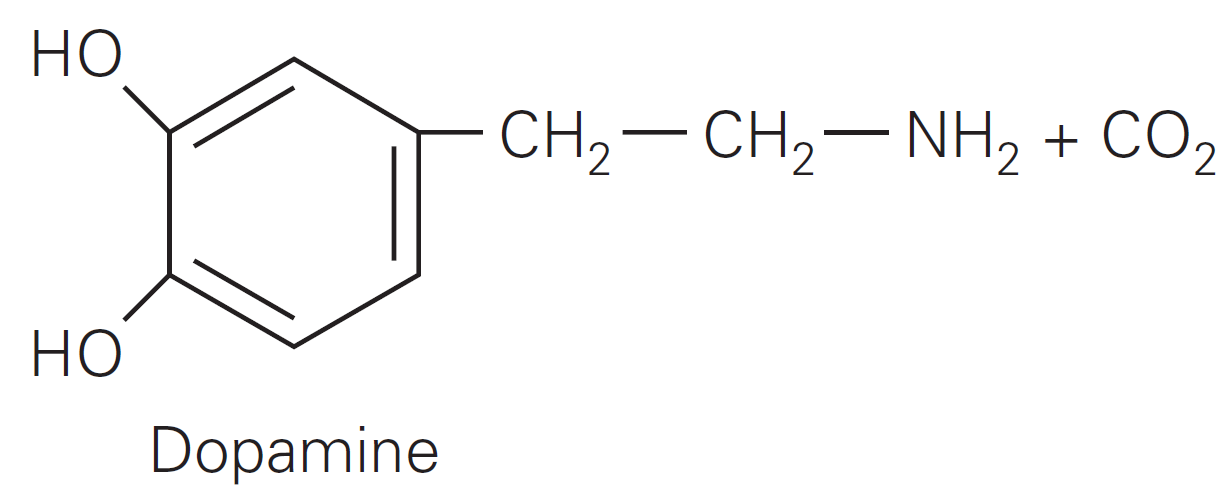
\includegraphics[width=0.5\textwidth]{pictures/Bilder_monoamine_systeme/dopamin.PNG}
    \caption[Dopamin]{\textbf{Dopamin.} Abbildung aus \textit{Principles of Neural Science}, Kandel et al. \textsuperscript{\cite[Kap.~13]{kandel2013principles}}.}
    \label{fig:dopamin}
\end{figure}{}

Eine Vielzahl dopaminerger Neurone sind in der Substantia nigra\index{Substantia nigra} (Abb.~\ref{fig:dopaminerge_kerngebiete}~A,B) des Mesencephalons lokalisiert.
Die Substantia nigra besteht aus zwei Teilgebieten. Eines davon ist die \textit{Substantia nigra pars compacta}. 
Aufgrund pigmentierter, Melanin-haltiger Neurone zeichnet sich dieses Kerngebiet durch eine dunklere Färbung aus.
Die dort lokalisierten dopaminergen Neurone projizieren in den Nucleus caudatus\index{Nucleus! caudatus} und das (Caudo-)Putamen\index{Putamen} der Basalganglia des Telencephalons \textsuperscript{\cite[Kap.~9]{crossman2014neuroanatomy}}.
Da beide Gebiete gemeinsam das Striatum bilden, werden diese Projektionen als \textbf{nigrostriatale Bahn} \index{Tractus! nigrostriatalis} bezeichnet.
Über die nigrostriatale Bahn üben die dopaminergen Neurone der Substantia nigra einen inhibitorischen Effekt auf das Striatums\index{Striatum} aus. Somit wirken sie inhibitorisch auf motorische Impulse des Großhirns.
Dadurch spielen sie eine wichtige Rolle für die Bewegungsinitiation \textsuperscript{\cite[Kap.~6]{trepel2011neuroanatomie}}.
Zudem sind sie an der Kontrolle von Willkürmotorik, Körperhaltung und Muskeltonus beteiligt. Die Degeneration dopaminerger Neurone der Substantia nigra pars reticulata führt zur Erkrankung Morbus Parkinson\index{Morbus Parkinson} \textsuperscript{\cite[Kap.~9]{crossman2014neuroanatomy}} und zu anderen motorischen Erkrankungen \textsuperscript{\cite[Kap.~13]{kandel2013principles}}.
Der unpigmentierte Bereich der Substantia nigra, die pars reticulata, ist als funktionelles Teilgebiet der Basalganglia (Kap.~\ref{subsec:Basalganglia}) ebenfalls in die Kontrolle der Motorik involviert \textsuperscript{\cite[Kap.~9]{crossman2014neuroanatomy}}.

\begin{figure}[H]
    \centering
    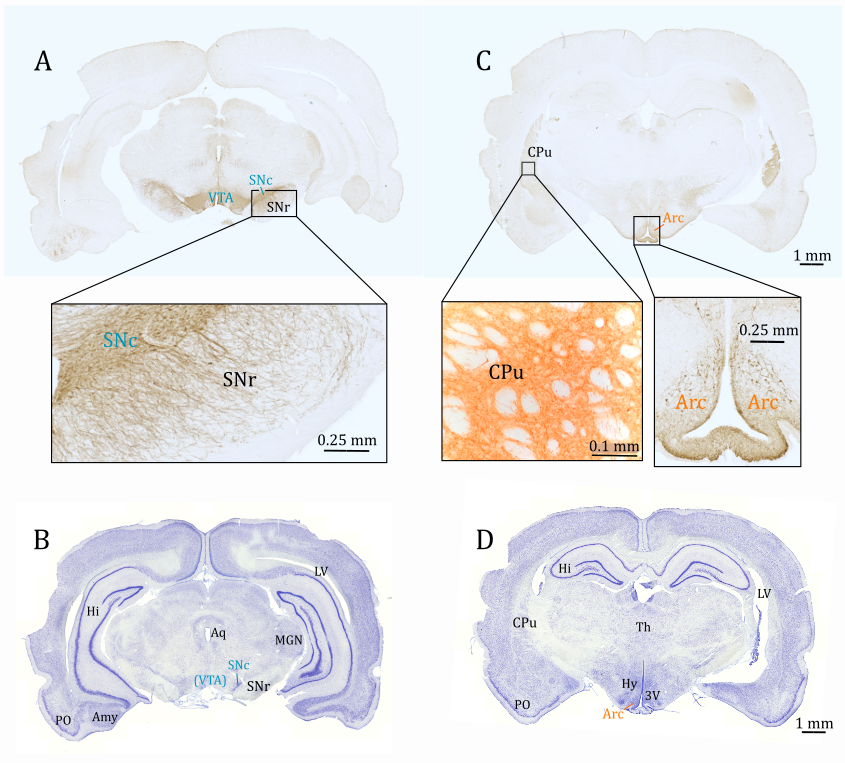
\includegraphics[width=\textwidth]{pictures/Bilder_monoamine_systeme/dopaminerge_kerne.png}
    \caption[Dopaminerge Kerngebiete]{\textbf{Dopaminerge Kerngebiete.} Nissl- (C,D) und immunohistochemische (Tyrosin-Hydroxylase-Nachweis) Schnitte (A,C) von caudal (A: Ia09-3, B: N18-1) nach rostral (C: Ib10-4, D: N21-4). Zu sehen sind die drei dopaminergen Kerngebiete: Die Substantia nigra pars compacta (SNc) und die Area tegmentalis ventralis (VTA) des Mesencephalons, sowie der Nucleus arcuatus (Arc) des Diencephalons. Einige der Projektionsgebiete, wie das (Caudo-)Putamen (CPu) des Striatums und die Substantia nigra pars reticulata (SNr), sind ebenfalls dargestellt. Das Putamen, als Teil der nigrostriatalen Bahn, erhält Projektionen aus der Substantia nigra pars compacta. Auch die Substantia nigra pars reticulata erhält Projektionen aus der pars compacta. Ebenfalls gekennzeichnet sind Areale des Telencephalons: Amygdala (Amy), Hippocampus (Hi), lateraler Ventrikel (LV), primärer olfaktorischer Cortex (PO). Bereiche des Diencephalons: dritter Ventrikel (3V), Hypothalamus (Hy), Nucleus geniculatum mediale (MGN), Thalamus (Th). Teilgebiete des Mesencephalons: Aquädukt (Aq).}
    \label{fig:dopaminerge_kerngebiete}
\end{figure}

Dorso-medial der Substantia nigra erstrecken sich dopaminerge Neurone, die die \textit{Area tegmentalis ventralis}\index{Area tegmentalis ventralis} (VTA) bilden (Abb.~\ref{fig:dopaminerge_kerngebiete}~A,B). Die dort lokalisierten dopaminergen Neurone bilden den Ausgangspunkt des aufsteigenden, mesolimbischen Traktes, sowie den mesocortikalen Trakt. Der \textbf{mesocortikale Trakt}\index{Tractus! mesocortikal} innerviert den präfrontalen Cortex. Der \textbf{mesolimbische Trakt}\index{Tractus! mesolimbisch} innerviert mehrere Teilgebiete des Vorderhins (Proencephalon), wie beispielsweise den cingulären Cortex und die Amygdala \textsuperscript{\cite[Kap.~9]{crossman2014neuroanatomy}}, sowie den Nucleus accumbens\index{Nucleus! accumbens} und den Nucleus caudatus\index{Nucleus! caudatus}.
Sowohl der mesolimbische als auch der mesocortikale Trakt sind zentrale Komponenten des Belohnungs-Schaltkreises \textsuperscript{\cite[Kap.~49]{kandel2013principles}}.
Des Weiteren spielen sie eine wichtige Rolle bei Emotionen, Aufmerksamkeit, Motivation \textsuperscript{\cite[Kap.~13]{kandel2013principles}} und der Regulation des Arbeitsgedächtnis. Fehler in der dopaminergen Regulation dieser beiden Systeme können mit Schizophrenie assoziiert werden \textsuperscript{\cite[Kap.~67]{kandel2013principles}}.
Auch an Rauschgiftsucht sind diese beiden Systeme beteiligt \textsuperscript{\cite[Kap.~13]{kandel2013principles}}.
\\
\\
Der vierte dopaminerge Trakt ist der \textbf{tuberoinfundibulare Trakt}\index{Tractus! tuberoinfundibular}. Er projiziert ausgehend von den dopaminergen Neuronen des \textit{Nucleus arcuatus} (Abb.~\ref{dopaminerges_system}~C,D) des diencephalen Hypothalamus zur Hypophyse\index{Hypophyse! allgemein}. Durch diese Projektion wird die Sekretion von Hormonen reguliert \textsuperscript{\cite[Kap.~13]{kandel2013principles}}.

\begin{figure}[H]
    \centering
    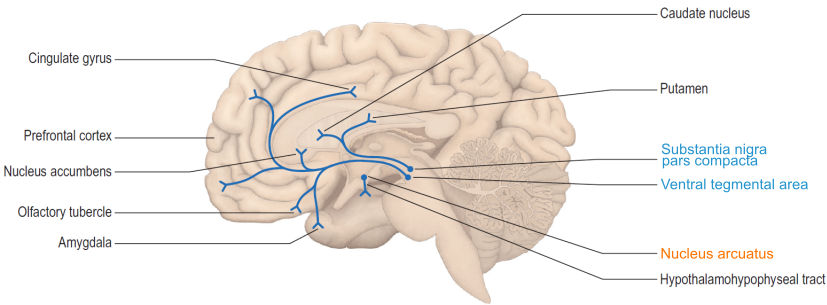
\includegraphics[width=\textwidth]{pictures/Bilder_monoamine_systeme/dopaminerges_system.PNG}
    \caption[Dopaminerges System]{\textbf{Dopaminerges System.} Zwei dopaminerge Kerngebiete, die Substantia nigra pars compacta und die Area tegmentalis ventralis, sind im Mesencephalon gelegen. Die dopaminergen Neurone des Nucleus arcuatus sind im Diencephalon lokalisiert. Abbildung nach \textit{Neuroanatomy}, Crossman und Neary
    \textsuperscript{\cite[Kap.~9]{crossman2014neuroanatomy}}.}
    \label{fig:dopaminerges_system}
\end{figure}
